\section{Serious Games}
Videospiele haben sich über die letzten Jahren zur beliebtesten und erfolgreichsten Form der Unterhaltung entwickelt. Die Videospielindustrie hat im Jahr 2017 mit 116 Milliarden Dollar mehr Umsatz generiert als Fernsehen, Filme und Musik zusammen. Die Verkäufe im Videospielsektor steigen jährlich um rund 10\%, während die Einnahmen der anderen Branchen fallen. Als Beispiel ist das Videospiel Grand Theft Auto V zu nennen, welches im Jahr 2013 erschienen ist und mittlerweile mehr als 90 Millionen Einheiten verkauft hat. Weiters hält es den Rekord, das meistverkaufte Produkt in der Unterhaltungsindustrie zu sein. \cite{reuters:2018:gaming} \\ 
Mit dem Aufstieg der Videospielindustrie hat sich ein interessanter Forschungsbereich in Bezug auf die medizinische Technik entwickelt. Der Begriff Serious Games wurde bereits 1984 von \citeauthor{c_abt:1987:serious_games} im Werk \enquote{Serious Games} erwähnt, wo der Autor beschreibt, dass Videospiele unter anderem im Bildungsbereich eingesetzt werden könnten \cite{c_abt:1987:serious_games}.
Die primären Märkte für Serious Games sind das Militär, die Regierung, das Bildungswesen, das Gesundheitswesen und Unternehmen. Regierungen, speziell das Militär sind die wichtigsten Quellen für die Finanzierung solcher Spiele. \cite{michael:2006:educate} \\
Jedoch existiert keine eindeutig anerkannte Definition des Begriffs. Allerdings besitzen die meisten Begriffsbestimmungen die gleiche Kernaussage, dass Serious Games Spiele seien, die für andere Zwecke eingesetzt werden, als reinen Zeitvertreib. Im Vergleich zu Videospielen, die den Spieler/innen die beste Erfahrung bieten wollen, versuchen Serious Games konkrete Probleme zu lösen und einen Lerneffekt zu erzielen. Zudem ist es wichtig, dass der Fokus auf das Lernen gelegt wird. Darüber hinaus müssen Annahmen für Simulationen korrekt sein, da ansonsten falsche Arten von Fähigkeiten vermittelt werden. In Videospielen wird oft zu verstehen gegeben, dass die Kommunikation zwischen Personen perfekt ist (keine Missverständnisse, Unterbrechungen, \dots), jedoch sollten lehrreiche Spiel verdeutlichen, dass Gespräche selten perfekt sind (Unterschiede zwischen Serious Games und Videospielen siehe Tabelle \ref{tab:serious_games_vs_entertainment_games}). \cite{serious_games:2007:an_overview}

\begin{table}[ht]
    \centering
    \begin{tabular}{|l|l|l|}
        \hline
        \rowcolor[rgb]{0.851,0.851,0.851}   & \textbf{Serious Games}                & \textbf{Videospiele} \\ 
        \hline
        Spielerfahrung           & Problemlösung                                    & Spielerfahrung \\ 
        \hline
        Fokus                    & Lernen                                           & Spaß \\ 
        \hline
        Simulationen             & \makecell[l]{Annahmen wichtig für \\ funktionierende Simulationen} & vereinfachte Simulationsprozesse \\ 
        \hline
        Kommunikation            & reflektiert natürliche Kommunikation             & Kommunikation ist perfekt \\
        \hline
    \end{tabular}
    \caption{Unterschiede zwischen Serious Games und Videospielen \cite{serious_games:2007:an_overview}}
	\label{tab:serious_games_vs_entertainment_games}
\end{table}

Kategorien von unterschiedlichen Lernspielen abzugrenzen, ist nicht einfach. \citeauthor{breuer_bente:2010:why_so_serious} haben verschiedene Lernspielkonzepte in Klassifikationen abgegrenzt. Abbildung \ref{fig:serious_games_relations} zeigt den Zusammenhang zwischen den unterschiedlichen Ansätzen, wie Entertainment Education, Game-based Learning, E-Learning, Serious Games, \ac{DGBL} und klassischen Edutainment Spiele. \cite{breuer_bente:2010:why_so_serious} \\
Edutainment bezeichnet jeden Versuch, das Lernen interessanter zu gestalten, egal in welchem Kontext \cite{michael:2006:educate}. Game-based Learning ist eine Unterkategorie, die Spiele für bildende Zwecke miteinbezieht (Brettspiele, Kartenspiele, Sport).
Serious Games haben auch Anwendungsgebiete außerhalb des Bildungssektors (Kunst, Therapie, Werbung, \dots). \ac{DGBL} ist eine Untermenge von Serious Games, welche hauptsächlich das Lernen in den Mittelpunkt stellen. E-Learning unterscheidet sich von diesen Kategorien, da es keine Beziehung zwischen Entertainment und Bildung bietet, sondern nur eine Kombination zwischen digitalen Medien und Lernen. \cite{breuer_bente:2010:why_so_serious} \\

\begin{figure}[h]
    \centering
	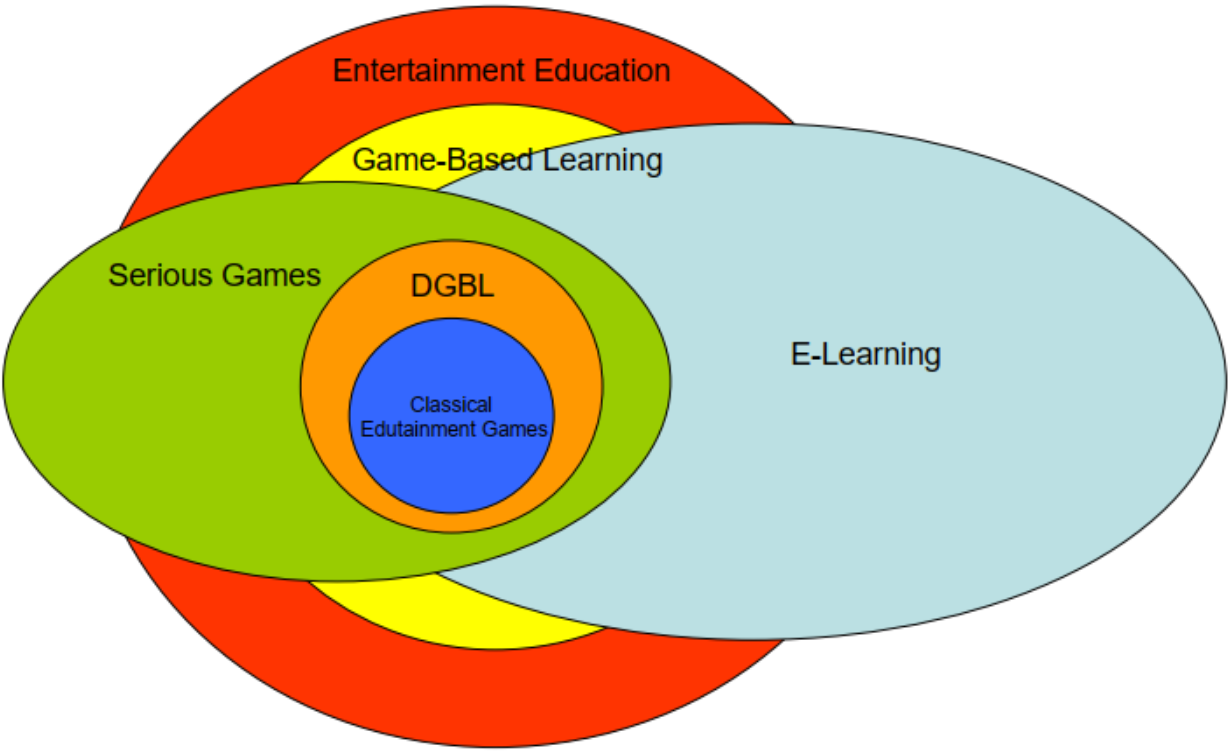
\includegraphics[width=1\linewidth]{figures/serious_games/serious_game_cat}
	\caption{Beziehungen zwischen Serious Games und ähnlichen Lernkonzepten \cite{breuer_bente:2010:why_so_serious}}
	\label{fig:serious_games_relations}
\end{figure}

% subsection{Spielen \& Lernen} todo dementia

\subsection{Spaß}
Ob ein Serious Game Spaß machen soll oder nicht ist keine einfache Frage. Viele Situationen, wie ein medizinischer Ernstfall, lassen sich nicht in ein spaßiges Spiel übertragen. Jedoch ist das wichtigste Argument für Spaß in Serious Games, dass Spieler/innen motiviert werden. \citeauthor{michael:2006:educate} haben in einer Umfrage einige Entwickler/innen, Pädagog/innen und Forscher/innen über die Wichtigkeit von Spaß in Serious Games befragt. Tabelle \ref{tab:serious_game_survey} zeigt die Ergebnisse der Untersuchung. Ein Großteil der Befragten hat angegeben, dass Unterhaltung wichtig oder sogar sehr wichtig ist. Keiner der 63 Partizipant/innen hat angegeben, dass Freude keine Rolle in Serious Games spielt. \cite{michael:2006:educate} \\
Wenn die Effekte und die Effektivität von Serious Games untersucht werden, dann muss laut \citeauthor{breuer_bente:2010:why_so_serious} die Wichtigkeit von Freude in die Forschung miteinbezogen werden. \cite{breuer_bente:2010:why_so_serious}
%todo

\begin{table}
    \centering
    \begin{tabular}{|l|l|} 
        \hline
        \rowcolor[rgb]{0.851,0.851,0.851} \textbf{Bedeutung}                & \textbf{Wichtigkeit}  \\ 
        \hline
        Sehr wichtig                      & 33,33\%               \\ 
        \hline
        Wichtig                           & 47,62\%               \\ 
        \hline
        Nützlich, aber kein primäres Ziel & 15,87\%               \\ 
        \hline
        Nicht so wichtig                  & 3,17\%                \\ 
        \hline
        Nicht wichtig                     & 0,00\%                \\
        \hline
    \end{tabular}
    \caption{Wichtigkeit von Spaß in Serious Games \cite{michael:2006:educate}}
	\label{tab:serious_game_survey}
\end{table}

\subsection{Wirkung}
Viele Tests an Patient/innen mit Einschränkungen oder Behinderungen zeigen, dass sich die motorischen Fähigkeiten mit einem Training, welches sich daran orientiert, ein konkretes Ziel zu erreichen, stark verbessern. Das Problem mit diesem Ansatz ist allerdings, dass den Patient/innen die Motivation fehlt, ständig wiederholende Tätigkeiten auszuführen. Computerspiele können eine positive Wirkung auf die Therapie haben, da sie die Aufmerksamkeit des/der Patient/in erfordern. Videospiele besitzen außerdem einen Schwierigkeitsgrad, der es dem/der Patient/in erlaubt, seinen/ihrer Fähigkeiten entsprechend zu spielen. Durch einen regulierbaren Schwierigkeitsgrad wird dem/der Behandelten nie langweilig, da das Spiel stets neue Herausforderungen bietet. Hinzukommend zum Lernaspekt, können Serious Games zusätzlich sehr motivierend sein, was förderlich für die \Gls{adherence} ist. \cite{burke:2009:optimising} \\
Die Forschung hat bereits gezeigt, dass Serious Games Vorteile in der Schlaganfallrehabilitation bieten. In einer Studie wurde ein Spiel, welches explizit für die Hemineglect Behandlung entwickelt wurde, untersucht. Das Experiment hat über eine Laufzeit von fünf Monaten eine positive Wirkung bei den Patient/innen und eine verbesserte Performance bei den Tests gezeigt. \cite{mainetti:2013:duckneglect} \\
In einer anderen Studie wurde die medizinische Auswirkung von einem \ac{VR} Gaming System in der Behandlung von Schlaganfallpatient/innen getestet. An der Unternehmnung nahmen acht Patient/innen, zusätzlich zur normalen Therapie, über zwölf Wochen hinweg teil, während acht andere Patient/innen in einer Kontrollgruppe getestet wurden. Am Ende zeigte die Serious Game Gruppe, im Gegensatz zur Kontrollgruppe, eine deutliche Verbesserung in verschiedenen Tests. \cite{cameirao:2011:virtual_reality} \\
\citeauthor{wouters:2009:practices} haben 28 Studien über die Effektivität von Serious Games überprüft und sind zu dem Ergebnis gekommen, dass Serious Games die Aneignung von Wissen und kognitiven Fähigkeiten verbessern können. Darüber hinaus scheinen sie vielversprechend für den Erwerb von motorischen Skills und einem positiven Wandel der Einstellung zu sein. Die Autoren haben die Forschungsergebnisse in einer Abbildung zusammengefasst (siehe Abbildung \ref{fig:serious_games_outcomes}), welche sich in folgende Kategorien einteilen lassen: kognitive Fähigkeiten, motorische Fähigkeiten, affektive Lernergebnisse, kommunikative Fähigkeiten. Allerdings gibt es laut \citeauthor{wouters:2009:practices} wenig Belege für die Steigerung der Motivation und der kommunikativen Fähigkeiten. \cite{wouters:2009:practices} \\ 
Weitere empirische Beweise für die positive Wirkung von Serious Games finden sich in der Literaturrecherche von \citeauthor{connolly:2012:systematic} bestehend aus insgesamt 129 wissenschaftlichen Arbeiten \cite{connolly:2012:systematic}. 

\begin{figure}[h]
    \centering
	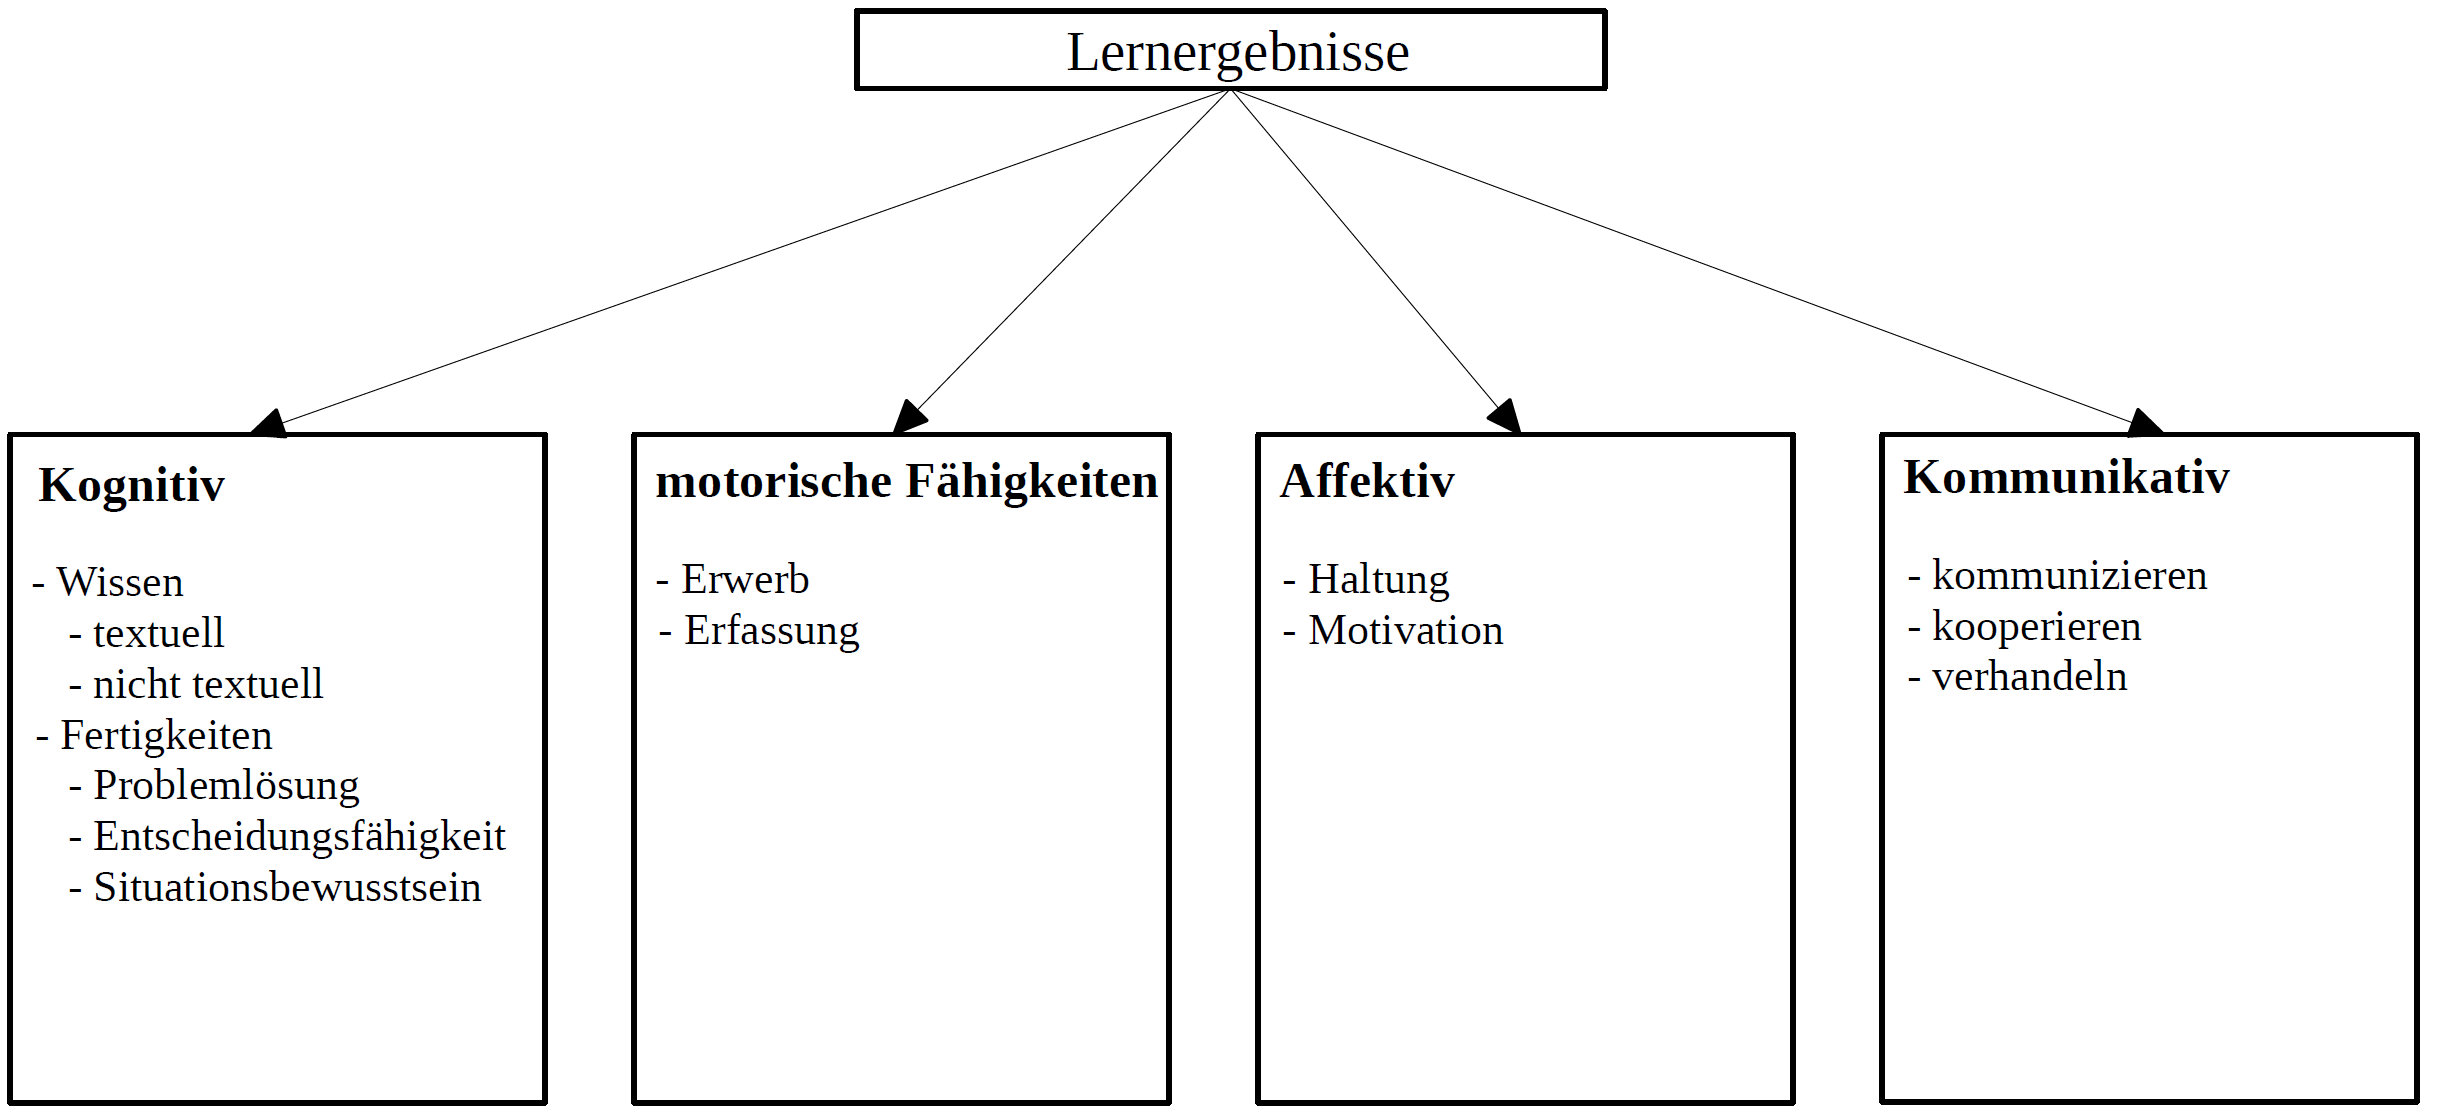
\includegraphics[width=0.8\linewidth]{figures/serious_games/learning_outcomes_deu}
	\caption{Lernerfolge mit Serious Games (aus dem Englischen nach \cite{wouters:2009:practices})}
	\label{fig:serious_games_outcomes}
\end{figure}

\subsection{Serious Games in der Rehabilitation}
Der Begriff Rehabilitation bezeichnet einen Wandel des Lebensstils als Antwort auf eine Krankheit oder ein traumatisches Erlebnis. Der Erfolg einer Rehabilitation beruht auf vielen verschiedenen Faktoren, wie Timing, Patient/innenauswahl, Wahl des Rehabilitationsprogramms, durchgehende medizinische Betreuung, \ac{etc.}. \cite{gunasekera:2005:rehabilitation} \\ %change
\citeauthor{flores:2008:IPM:1501750.1501839} recherchierten in Journalen und Datenbanken, um eine Menge von Kriterien herauszuarbeiten, die wichtig sind, um ein Serious Game für die Schlaganfallrehabilitation zu entwickeln. Die Literatur wurde dahingehend untersucht, um eine effektive Therapie für Schlaganfallpatient/innen sowie Kriterien für die Unterhaltung der älteren Bevölkerung, zu finden. In der Tabelle \ref{tab:criteria_serious_games} ist die Menge der herausgearbeiteten Kriterien dargestellt. Ein perfektes Serious Games für die Schlaganfallrehabilitation würde alle Kriterien erfüllen. \cite{flores:2008:IPM:1501750.1501839} 

% \usepackage{colortbl}


\begin{table}
\centering
\begin{tabular}{|l|l|} 
\hline
\rowcolor[rgb]{0.851,0.851,0.851}  \textbf{Kriterien für Schlaganfallrehabilitation}  & \begin{tabular}[c]{@{}>{\cellcolor[rgb]{0.851,0.851,0.851}}l@{}}\textbf{Kriterien für die Unterhaltung von } \\ \textbf{älteren Personen} \end{tabular}  \\ 
\hline
Anpassbarkeit an den Skilllevel                                                       & kognitive Herausforderung                                                                                                                                \\ 
\hline
sinnvolle Aufgaben                                                                    & einfache Zielsetzung/Oberfläche                                                                                                                          \\ 
\hline
angemessenes Feedback                                                                 & motivierendes Feedback                                                                                                                                   \\ 
\hline
geeignete ROM                                                                         & soziale Aktivität                                                                                                                                        \\ 
\hline
Fokus von der Übung abgelenken                                                        & schaffen von neuem Wissen                                                                                                                                \\ 
\hline 
& \begin{tabular}[c]{@{}l@{}}Feingefühl für reduzierte sensorische \\ Fähigkeiten und langsamere Reaktionszeiten \end{tabular}                             \\
\hline
\end{tabular}
\caption{Designkriterien für Schlaganfallrehabilitationsprogramme \cite{flores:2008:IPM:1501750.1501839}}
\label{tab:criteria_serious_games}
\end{table}

Eine erfolgreiche Rehabilitation erfordert, dass sich das Spiel an die Fähigkeiten des/der Patient/in anpasst. Daher sollte sich der Schwierigkeitsgrad mit dem Fortschritt der behandelten Person ebenfalls steigern. Sinnvolle Aufgaben sollten eingebaut werden, damit der/die Patient/in eine direkte Verbindung zwischen der Therapie und alltäglichen Aktivitäten sieht. Das Spiel sollte Feedback für Patient/in und Therapeut/in bieten. Aus den Ergebnissen sollte ersichtlich sein, wie sich der/die Patient/in über die Zeit hinweg verbessert. Aus den Rückmeldungen des Serious Games sollte der zukünftige Therapieweg ablesbar sein. \cite{flores:2008:IPM:1501750.1501839}

Beim Vergleich von Bildungsspielen und Entertainmentspielen kam \citeauthor{flores:2008:IPM:1501750.1501839} auf das Ergebnis, dass therapeutischen Spielen Unterhaltungsqualitäten fehlen und Unterhaltungsspielen fehlt es an eingebauten therapeutischen Maßnahmen für die Rehabilitation. \cite{flores:2008:IPM:1501750.1501839}


